\chapter{Árboles}

Los árboles son un caso especial de grafo. Principalmente, un árbol es un grafo que cumple las siguientes propiedades:

\begin{itemize}
	\item Es conexo.
	\item No tiene ciclos.
	\item Tiene \(V-1\) aristas, dónde \(V\) es él número de vértices.
\end{itemize}

Es decir, son grafos que se ven de la siguiente manera:

\begin{center}
	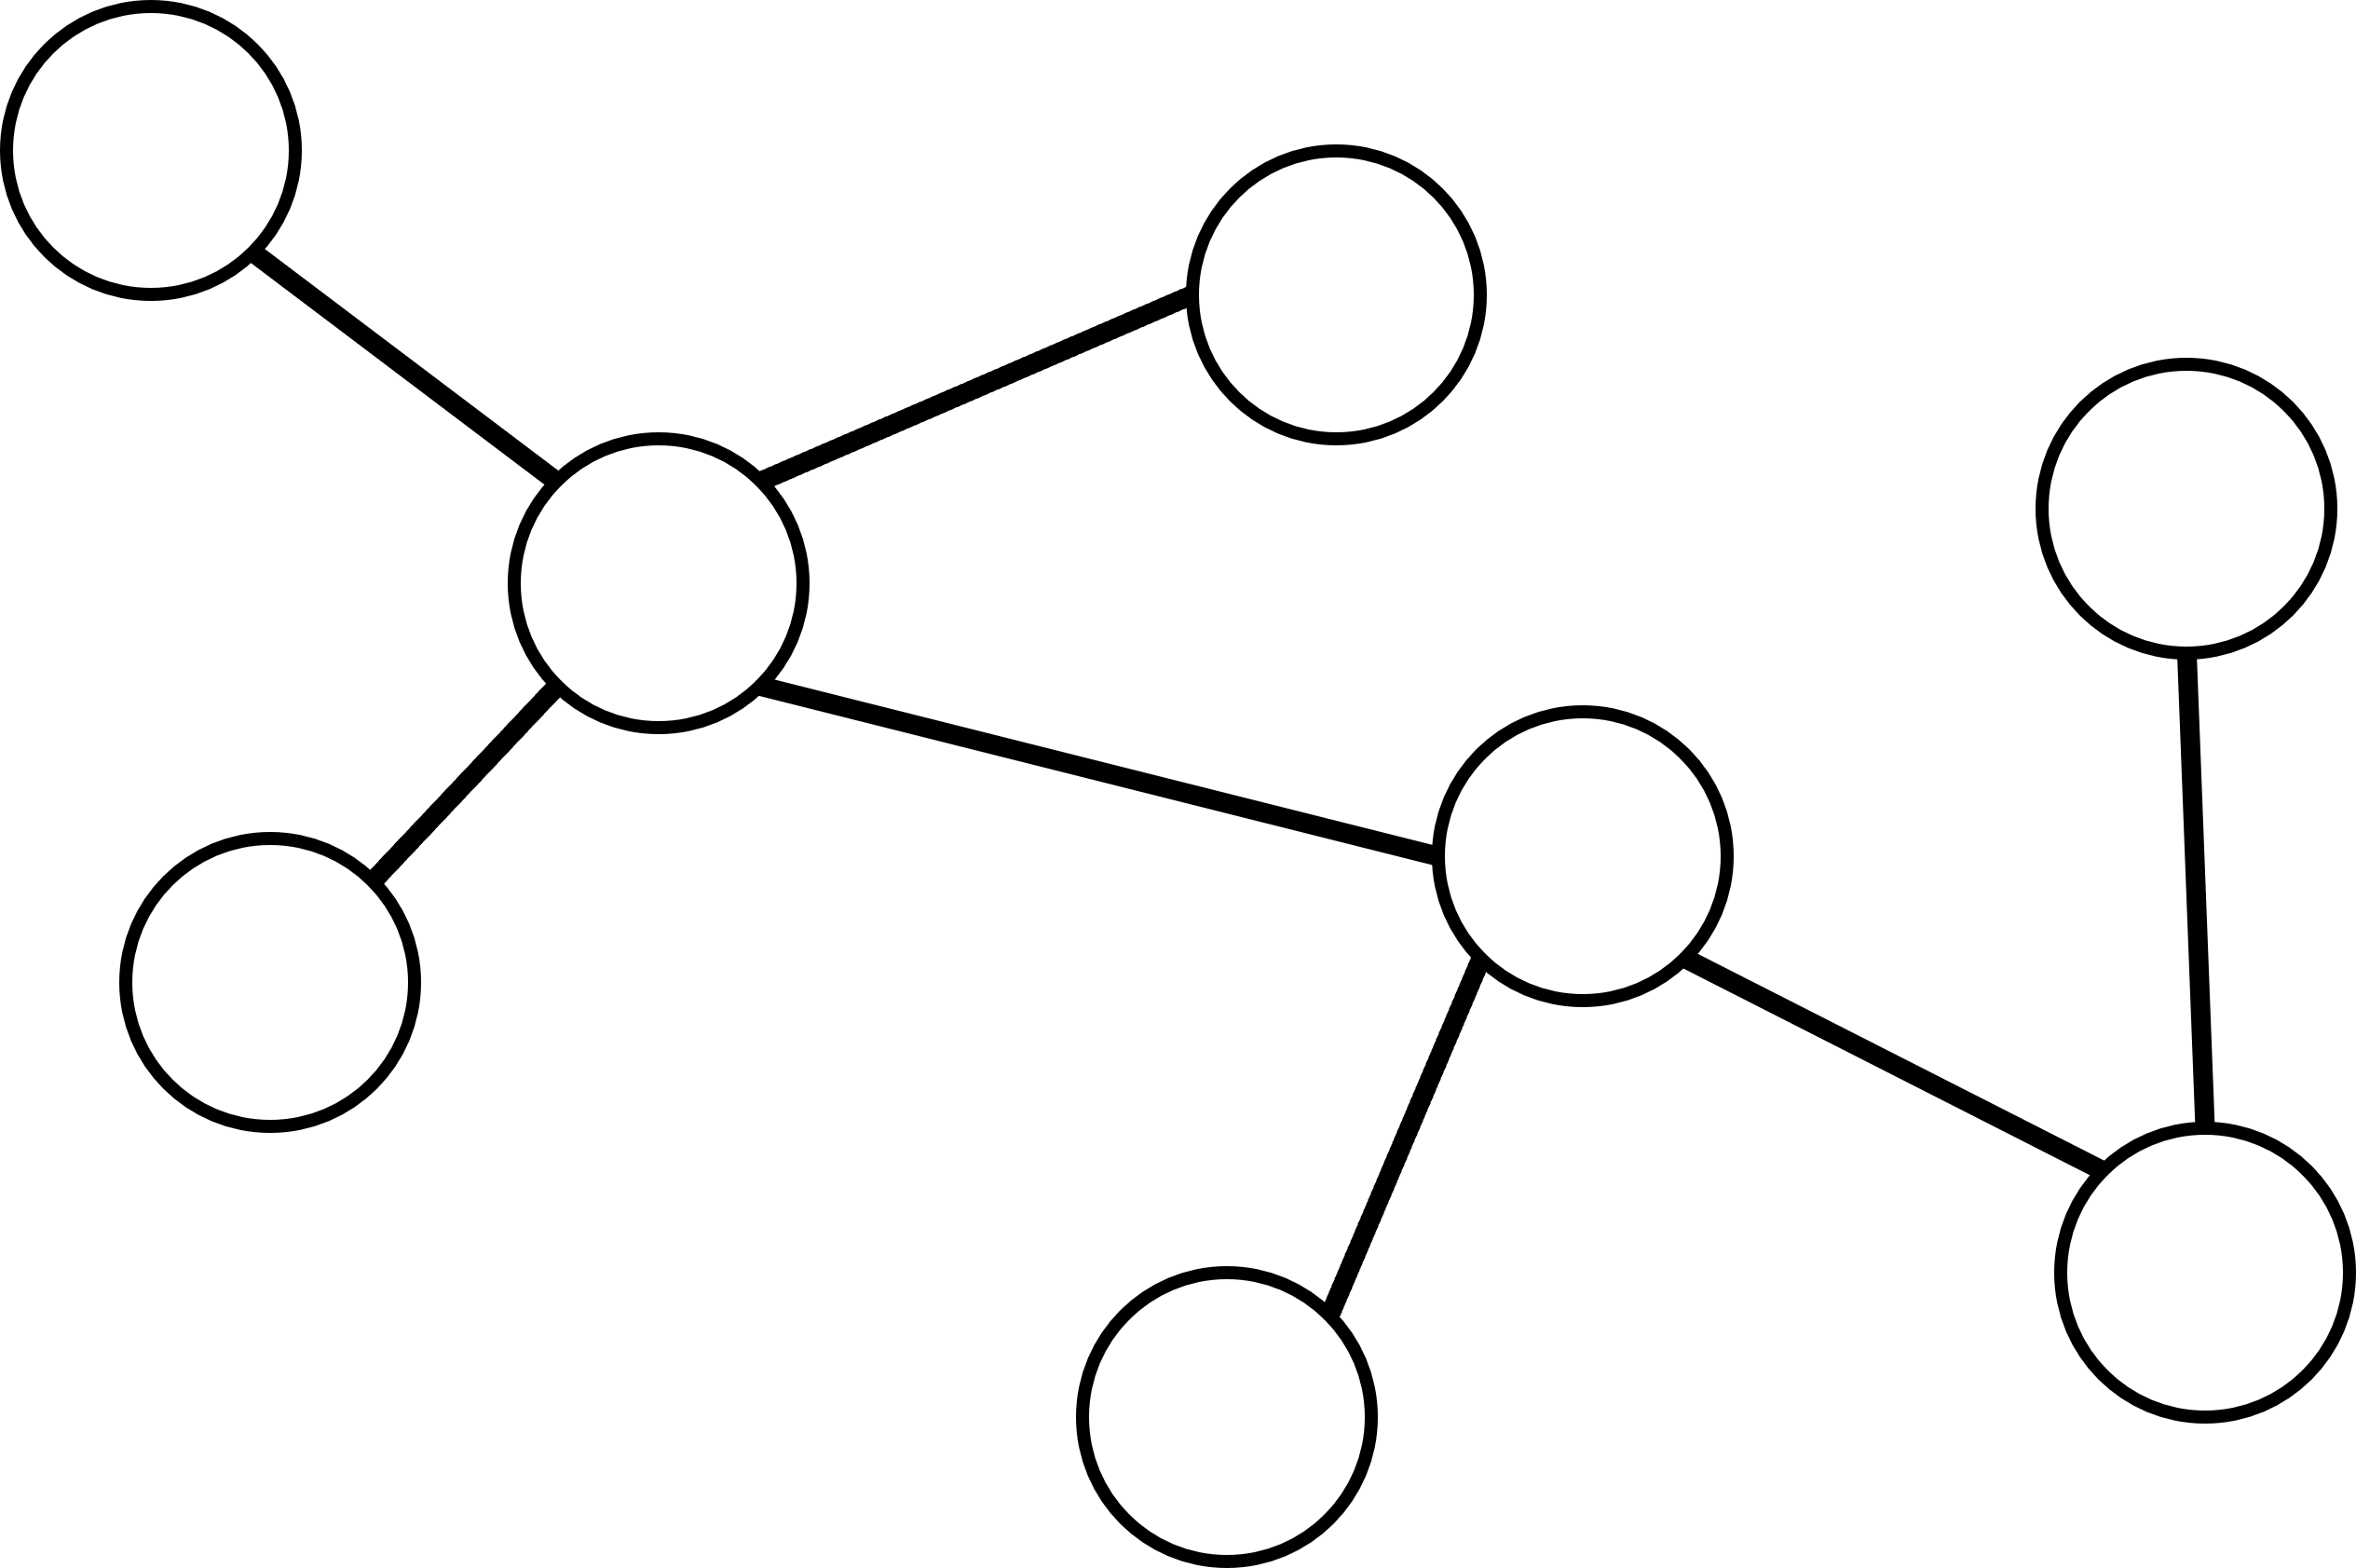
\includegraphics[scale=0.25]{arboles/arbol}
\end{center}

Una de las propiedades más importantes que se obtiene en un árbol es que es un grafo en el que para todo par de vértice existe un único camino simple. Siempre, elige dos vértices y habrá exactamente un camino entre los dos. 

\section{Árboles enraizados}
Es común que los árboles tienen un nodo especial llamado raíz. Normalmente cuando tenemos una raíz, dibujamos el árbol a partir de la raíz, por ejemplo:

\begin{center}
	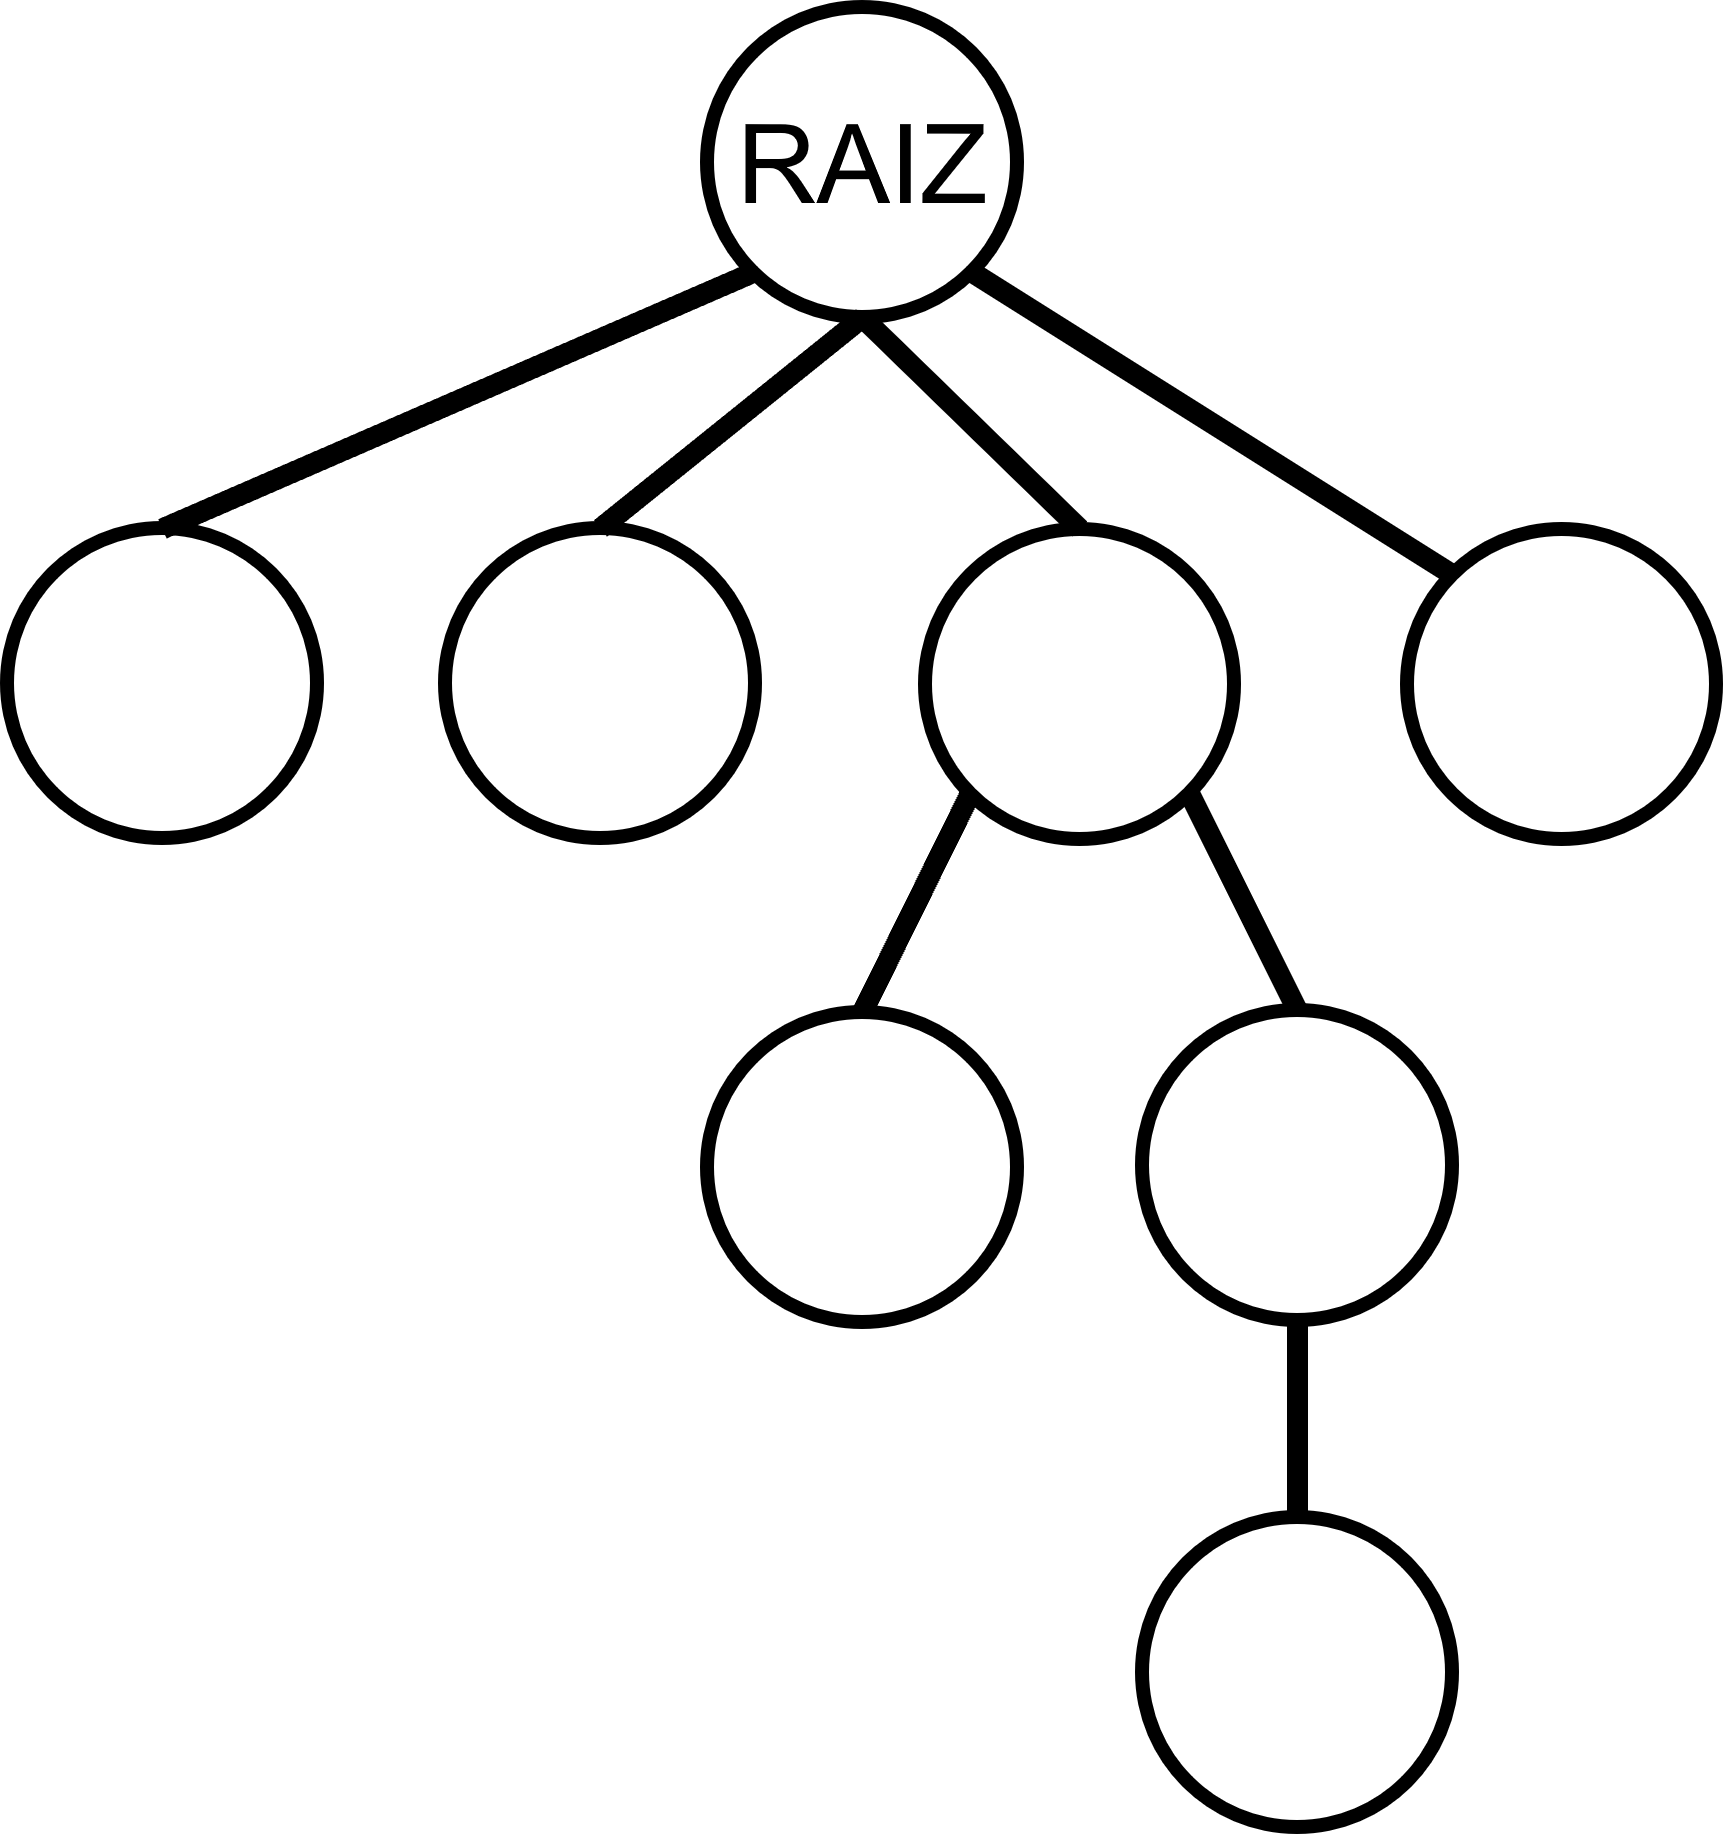
\includegraphics[scale=0.33]{arboles/raiz}
\end{center}

La asignación de la raíz nos permite hacer otras definiciones. 


Los vecinos de un vértice se parten en dos tipos dependiendo de su relación con respecto a la raíz:
\begin{itemize}
	
\item \textbf{Padre:} Todo vértice tiene un vecino llamado padre, excepto por la raíz que no tiene. El padre de un vértice es aquel vecino al cual te tienes que mover para acercarte a la raíz, normalmente el padre se encuentra arriba en el dibujo.

\item \textbf{Hijos:} Los vecinos que se alejan de la raíz son los hijos, en el dibujo los hijos de un vértice se encuentran por debajo. 
\end{itemize}

